\documentclass[conference]{IEEEtran}
\IEEEoverridecommandlockouts

\usepackage{cite}
\usepackage{amsmath,amssymb,amsfonts}
\usepackage{graphicx}
\usepackage{textcomp}
\usepackage{xcolor}
\usepackage{booktabs}
\usepackage{url}
\usepackage{tikz}
\usetikzlibrary{arrows.meta,positioning,calc}

\def\BibTeX{{\rm B\kern-.05em{\sc i\kern-.025em b}\kern-.08em
    T\kern-.1667em\lower.7ex\hbox{E}\kern-.125emX}}

\begin{document}

\title{Intelligent Discovery of Photos in an Event through Face Recognition:\\
A Selfie-Driven, Liveness-Gated Retrieval System}

\author{\IEEEauthorblockN{Nandalal Shukla}
\IEEEauthorblockA{\textit{[Department / Programme]}, \textit{[Institution]}\\
\textit{[City, Country]}\\
shuklanandalal@gmail.com}}

\maketitle

% =====================================================================================
\begin{abstract}
Event photographers deliver thousands of pictures, yet each guest wants only the few in which they appear. Manual sorting does not scale, and one shared album exposes every guest's photos to anyone who holds the link. This paper presents PhotoMatch AI, an end-to-end system in which an organizer uploads an album once and each guest retrieves a private gallery of their own photos by sending a single selfie to a Telegram or WhatsApp bot. Faces are detected with SCRFD, described by 512-dimensional ArcFace embeddings and compared by cosine similarity inside PostgreSQL with the pgvector extension, which also serves as the job queue, so no separate vector database or message broker is required. For private events, an optional liveness gate combines a guided head turn, a same-person check, a passive anti-spoofing ensemble and a match against the original selfie before any photo is shown. We evaluate the shipped implementation on a four-core CPU. In a controlled nine-identity perturbation study the embeddings stayed above the 0.45 decision threshold under strong blur, compression, darkness, noise and rotation, and no false match occurred in 3{,}280 cross-identity comparisons (largest similarity 0.238). Exact event-scoped search took 2.1\,ms for 1{,}000 faces and 24\,ms for 10{,}000 faces and was almost independent of table size (16 to 23\,ms when the table grew tenfold), whereas an HNSW index retrieved at most 93\% of the true matches at 250{,}000 faces. We state plainly what is not yet evaluated: standard face benchmarks and a labelled presentation-attack protocol are left for future work.
\end{abstract}

\begin{IEEEkeywords}
face recognition, photo retrieval, liveness detection, presentation attack detection, vector search, pgvector, ArcFace
\end{IEEEkeywords}

% =====================================================================================
\section{Introduction}
A wedding, a conference or a college festival produces thousands of photographs within a few hours. A few days later the album is ready, and the organizer becomes a human search engine: relatives and friends write to ask for ``the pictures with me''. Two workarounds are common, and both are unsatisfying. Sending photos one person at a time consumes hours of the organizer's attention, while publishing a single album link delivers everything to everyone and gives guests no way to keep their image private. The underlying task is simple to state---\emph{given one picture of a person, find that person in a large collection}---and it is exactly the task that deep face recognition now solves with high reliability on public benchmarks \cite{taigman2014,schroff2015,deng2022arcface,wang2021survey}.

Commercial event-photo platforms already advertise selfie-based search, in one case with a liveness check in front of the search \cite{kamero,picsolv}. To our knowledge there is no peer-reviewed description of how such a service is built or how it behaves, so its design trade-offs and failure modes remain undocumented. Building one raises four practical questions. \emph{(i) Cost shape:} indexing is bursty (tens of thousands of faces within hours, then idle), so infrastructure should be light enough to run on a single small server. \emph{(ii) Privacy:} face embeddings are biometric templates \cite{mai2019reconstruction,gdpr}, and a forwarded gallery link must not reveal photos to the person who received it. \emph{(iii) Reach:} guests are non-technical and will not install an application or create an account, so the interaction must happen in the messengers they already use. \emph{(iv) Usability of liveness:} a liveness check that fails real people at the exact moment they want their photos is worse than none.

\textbf{Contributions.} This paper describes and evaluates PhotoMatch AI, an open implementation built to answer those questions:
\begin{enumerate}\setlength{\itemsep}{0pt}\setlength{\topsep}{2pt}
\item an architecture that keeps relational data, face vectors and the job queue in \emph{one} PostgreSQL database, uploads photos directly from the browser to object storage, and runs all neural networks in a stateless, CPU-only service;
\item an \emph{event-scoped exact} cosine search, justified empirically against HNSW indexing, including a post-filtering failure mode that we reproduce;
\item a liveness-gated delivery protocol that binds a gallery link to the live face of the person who sent the selfie, using a guided head-turn challenge with burst capture, a same-person check, a passive anti-spoofing ensemble and identity matching;
\item a dependency-light ONNX Runtime port of the detection, alignment, embedding and head-pose stages that installs from binary wheels on Windows, macOS and Linux; and
\item a measurement study of cost, robustness and scale on commodity hardware, with an explicit account of what the evidence does \emph{not} show.
\end{enumerate}
\noindent Section~\ref{sec:related} reviews related work, Section~\ref{sec:problem} formalizes the task, Sections~\ref{sec:arch}--\ref{sec:liveness} present the system, Section~\ref{sec:eval} reports the evaluation, and Sections~\ref{sec:discussion} and~\ref{sec:conclusion} discuss limits and conclude.

% =====================================================================================
\section{Related Work}\label{sec:related}
\subsection{Deep face recognition}
Early recognition relied on holistic projections such as Eigenfaces \cite{turk1991} and hand-crafted texture descriptors such as local binary patterns \cite{ahonen2006}. Deep networks changed the picture: DeepFace reported 97.35\% verification accuracy on Labeled Faces in the Wild (LFW) \cite{taigman2014,huang2007lfw}, VGG-Face showed that a standard deep network trained on a carefully curated dataset is competitive \cite{parkhi2015}, FaceNet learned a compact Euclidean embedding with a triplet loss and reached 99.63\% \cite{schroff2015}, and margin-based softmax losses---SphereFace, CosFace and ArcFace---made embeddings more discriminative on the hypersphere \cite{liu2017sphereface,wang2018cosface,deng2019arcface,deng2022arcface}. Residual networks \cite{he2016resnet}, large training sets such as WebFace260M \cite{zhu2021webface260m} and efficient large-scale training \cite{an2022partialfc} followed; comprehensive surveys are available \cite{wang2021survey}. LFW is now close to saturation, so harder protocols such as IJB-C are used to compare modern models \cite{maze2018ijbc,huang2014lfw}. Lightweight networks for mobile deployment \cite{chen2018mobilefacenets} show that accuracy and cost can be traded, but our setting is a server that processes an album in the background and can afford a ResNet-50 recognizer.

\subsection{Face detection, alignment and head pose}
Cascades \cite{viola2001} gave way to multi-task convolutional detectors \cite{zhang2016mtcnn}, single-shot detectors with landmark supervision \cite{deng2020retinaface} and compute-efficient designs such as SCRFD \cite{guo2022scrfd}, evaluated on WIDER FACE \cite{yang2016widerface}. Event photographs contain many small faces, which motivates scale-aware detection \cite{hu2017tinyfaces}. Recognition networks expect faces aligned to a canonical template, which is obtained from detected landmarks with a similarity transform \cite{umeyama1991}. Head pose can be derived from dense or 3-D landmarks \cite{bulat2017,murphy2009}; we use it to verify a head-turn challenge.

\subsection{Liveness and presentation attack detection}
Presentation attack detection (PAD) is standardized in ISO/IEC 30107-3 \cite{iso30107}. Early software countermeasures looked for involuntary motion such as eye blinks \cite{pan2007blink} or the motion of face parts \cite{kollreider2009}, or for texture differences between real skin and prints and screens \cite{chingovska2012,boulkenafet2016}. Datasets such as CASIA-FASD, OULU-NPU and CelebA-Spoof enabled deep PAD with auxiliary depth or remote-photoplethysmography supervision \cite{zhang2012casia,boulkenafet2017oulu,zhang2020celebaspoof,liu2018aux} and central-difference convolutions \cite{yu2020cdcn}; a survey is given in \cite{yu2023survey}. Passive models generalize imperfectly across cameras and attack types \cite{yu2023survey}, which is why challenge--response and passive checks are often combined. Digital manipulation and injection attacks, which bypass the camera, are a separate and growing threat \cite{tolosana2020}. We use the MiniFASNet ensemble released under the Apache-2.0 license by Minivision \cite{minivision} and pair it with an active head-turn challenge.

\subsection{Person search in photo collections}
Research on personal photo albums addresses recognition when faces are small, occluded or turned away \cite{zhang2015piper,oh2015person} and groups unlabeled faces by clustering \cite{wang2019linkage}. Our problem is narrower and query-driven: a guest supplies one frontal selfie and the system must return every photo of that person in one event, with privacy controls that photo-organizing tools do not need.

\subsection{Vector search}
Approximate nearest-neighbor methods such as HNSW graphs \cite{malkov2020hnsw}, product quantization \cite{jegou2011pq} and GPU libraries \cite{johnson2019faiss} make billion-scale search feasible. The \texttt{pgvector} extension brings exact and HNSW search into PostgreSQL \cite{pgvector}. Recent releases add iterative scans because index scans combined with a filter can return too few rows \cite{pgvector08}; we measure that effect in Section~\ref{sec:eval}.

\subsection{Privacy and fairness}
Deep templates can be inverted to recover recognizable face images \cite{mai2019reconstruction}, so stored embeddings are sensitive. Biometric data is a special category under the GDPR \cite{gdpr}. Recognition error rates differ across demographic groups \cite{buolamwini2018,grother2019frvt}. We return to these points in Section~\ref{sec:discussion}.

% =====================================================================================
\section{Problem Statement and Design Goals}\label{sec:problem}
Let an event $E$ consist of photos $P=\{p_1,\dots,p_N\}$. A detector finds a set of faces $F(p)$ in each photo, and an embedding function $\phi$ maps an aligned face crop to a unit vector in $\mathbb{R}^{512}$. A guest submits a selfie $s$ whose single main face yields the query $q=\phi(s)$. The system returns
\begin{equation}
R(q)=\Big\{\,p\in P_{\mathrm{approved}} \;:\; \max_{f\in F(p)} q^{\top}\phi(f)\;\ge\;\tau\,\Big\},
\label{eq:match}
\end{equation}
ranked by the maximum similarity, with $\tau=0.45$ in the deployed configuration. Only the best face per photo matters, because a guest appears in a photo at most once. Photos contributed by third parties are excluded from $R(q)$ until the organizer approves them.

We derived six goals from the scenario in the introduction.
\textbf{G1~Privacy:} selfies are never persisted, galleries are reachable only through a per-search link, and an organizer can switch guest access off at any time.
\textbf{G2~Scale:} thousands of photos and tens of thousands of faces per event.
\textbf{G3~Low operating cost:} one small server, no GPU, as few moving parts as possible.
\textbf{G4~Reach:} Telegram and WhatsApp, no app or account for guests.
\textbf{G5~Optional liveness:} for private events, only the person who sent the selfie may open the gallery.
\textbf{G6~Portability:} installable on a student laptop without a C++ toolchain.

% =====================================================================================
\section{System Architecture}\label{sec:arch}
\subsection{Components}
Figure~\ref{fig:arch} shows the system. A React single-page application serves organizers and guests. A Node.js API (Express 5, Prisma, better-auth) handles authentication, events, signed uploads, bot webhooks and gallery access, and serves the compiled web application in production so that browser and API share one origin. A background worker consumes jobs from a queue implemented with pg-boss \cite{pgboss} on PostgreSQL. A stateless Python service (FastAPI with ONNX Runtime \cite{onnxruntime}) is the only component that runs neural networks and never touches the database. PostgreSQL stores users and sessions, events, photos, face vectors (\texttt{vector(512)}) and the queue. Photo files live in an external object store (Cloudinary).

\begin{figure*}[!t]
\centering
\resizebox{0.97\textwidth}{!}{% System architecture (double-column figure). Absolute coordinates (cm) keep every arrow orthogonal.
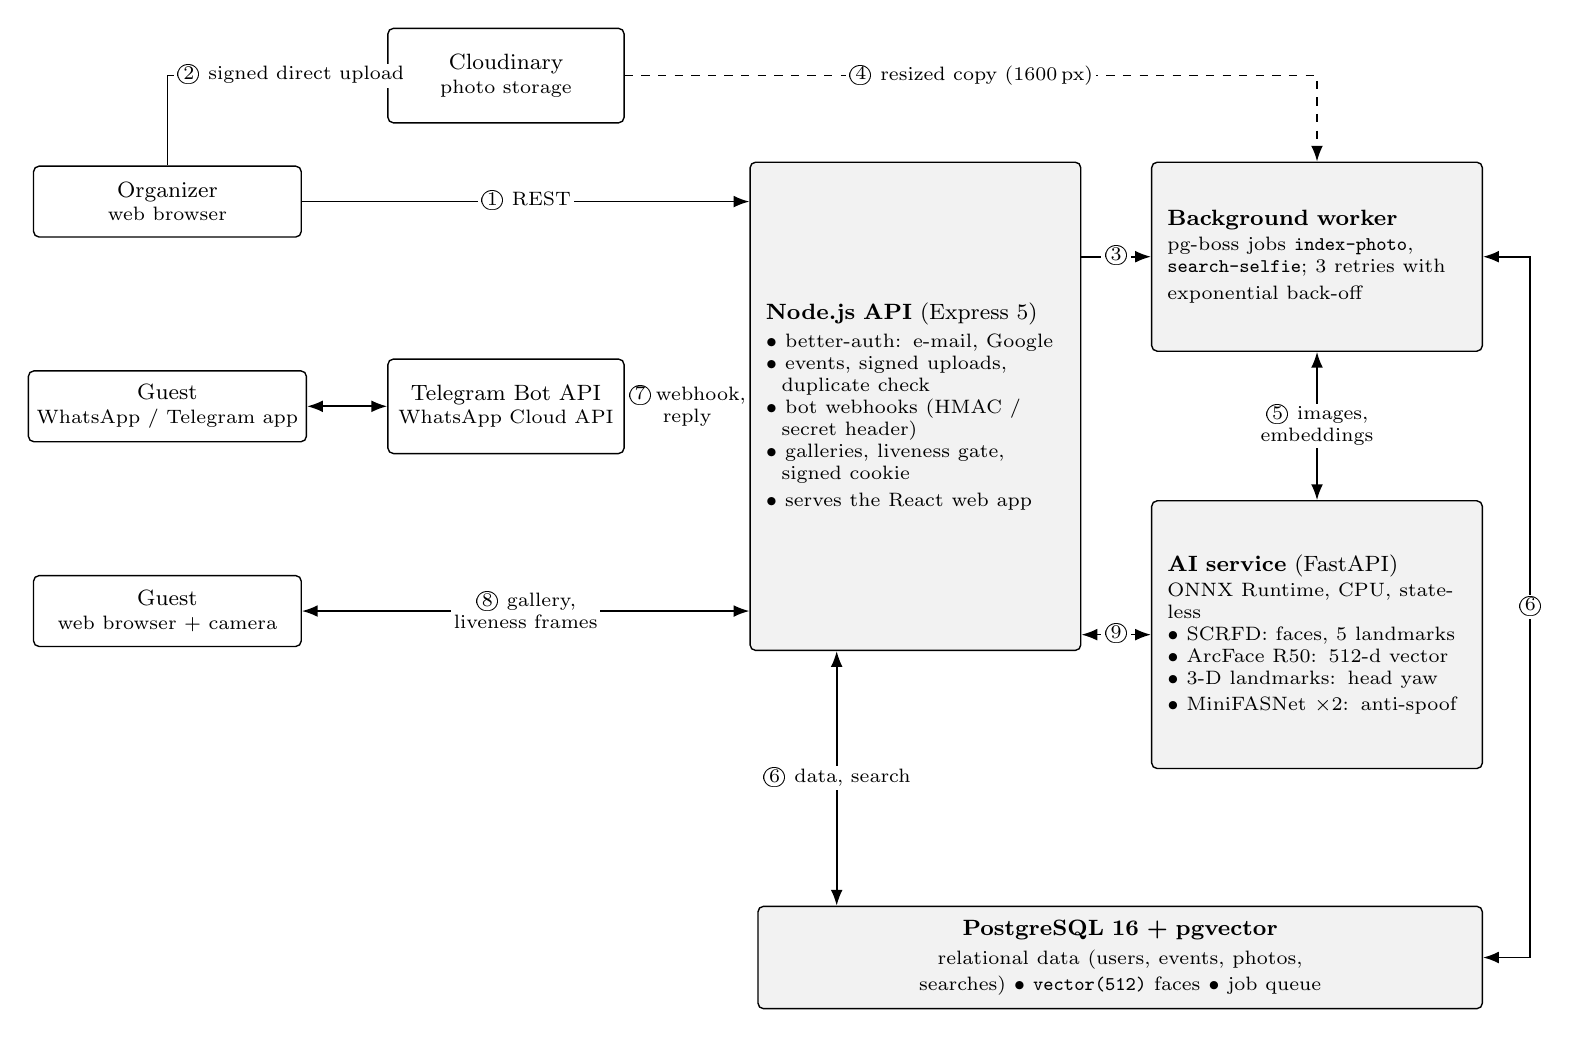
\begin{tikzpicture}[
  font=\footnotesize, >=Latex,
  box/.style={draw, rounded corners=2pt, align=center, inner sep=3pt, fill=white, line width=0.5pt, minimum height=9mm},
  svc/.style={box, fill=gray!10, align=left},
  lab/.style={font=\scriptsize, fill=white, inner sep=1pt, align=center},
  flow/.style={->, line width=0.6pt},
  two/.style={<->, line width=0.6pt}]

% ---- clients
\node[box, minimum width=34mm] (org) at (0,5.0)  {Organizer\\[-1pt]\scriptsize web browser};
\node[box, minimum width=34mm] (gm)  at (0,2.4)  {Guest\\[-1pt]\scriptsize WhatsApp / Telegram app};
\node[box, minimum width=34mm] (gb)  at (0,-0.2) {Guest\\[-1pt]\scriptsize web browser + camera};

% ---- external services
\node[box, minimum width=30mm, minimum height=12mm] (cld) at (4.3,6.6) {Cloudinary\\[-1pt]\scriptsize photo storage};
\node[box, minimum width=30mm, minimum height=12mm] (msg) at (4.3,2.4) {Telegram Bot API\\[-1pt]\scriptsize WhatsApp Cloud API};

% ---- application tier
\node[svc, minimum width=42mm, minimum height=62mm, text width=38mm] (api) at (9.5,2.4)
  {\textbf{Node.js API} (Express 5)\\[2pt]
   \scriptsize $\bullet$ better-auth: e-mail, Google\\
   \scriptsize $\bullet$ events, signed uploads,\\\scriptsize\ \ duplicate check\\
   \scriptsize $\bullet$ bot webhooks (HMAC /\\\scriptsize\ \ secret header)\\
   \scriptsize $\bullet$ galleries, liveness gate,\\\scriptsize\ \ signed cookie\\
   \scriptsize $\bullet$ serves the React web app};
\node[svc, minimum width=42mm, minimum height=24mm, text width=38mm] (wrk) at (14.6,4.3)
  {\textbf{Background worker}\\[1pt]
   \scriptsize pg-boss jobs \texttt{index-photo},\\
   \scriptsize \texttt{search-selfie}; 3 retries with\\
   \scriptsize exponential back-off};
\node[svc, minimum width=42mm, minimum height=34mm, text width=38mm] (ai) at (14.6,-0.5)
  {\textbf{AI service} (FastAPI)\\[1pt]
   \scriptsize ONNX Runtime, CPU, stateless\\
   \scriptsize $\bullet$ SCRFD: faces, 5 landmarks\\
   \scriptsize $\bullet$ ArcFace R50: 512-d vector\\
   \scriptsize $\bullet$ 3-D landmarks: head yaw\\
   \scriptsize $\bullet$ MiniFASNet $\times 2$: anti-spoof};

% ---- database
\node[svc, minimum width=92mm, minimum height=13mm, text width=88mm, align=center] (db) at (12.1,-4.6)
  {\textbf{PostgreSQL 16 + pgvector}\\[1pt]
   \scriptsize relational data (users, events, photos, searches) $\bullet$ \texttt{vector(512)} faces $\bullet$ job queue};

% ---- flows
\draw[flow] (org.east) -- node[lab, pos=0.5] {\textcircled{\scriptsize 1} REST} (api.west |- org.east);
\draw[flow] (org.north) |- node[lab, pos=0.78] {\textcircled{\scriptsize 2} signed direct upload} (cld.west);
\draw[two]  (gm.east) -- (msg.west);
\draw[two]  (msg.east) -- node[lab, pos=0.5] {\textcircled{\scriptsize 7}\,webhook,\\reply} (api.west |- msg.east);
\draw[two]  (gb.east) -- node[lab, pos=0.5] {\textcircled{\scriptsize 8} gallery,\\liveness frames} (api.west |- gb.east);
\draw[flow] (api.east |- wrk.west) -- node[lab, pos=0.5] {\textcircled{\scriptsize 3}} (wrk.west);
\draw[flow, dashed] (cld.east) -- node[lab, pos=0.5] {\textcircled{\scriptsize 4} resized copy (1600\,px)} (wrk.north |- cld.east) -- (wrk.north);
\draw[two]  (wrk.south) -- node[lab, pos=0.5] {\textcircled{\scriptsize 5} images,\\embeddings} (ai.north);
\draw[two]  (api.east |- ai.west) -- node[lab, pos=0.5] {\textcircled{\scriptsize 9}} (ai.west);
\draw[two]  ([xshift=-10mm]api.south) -- node[lab, pos=0.5] {\textcircled{\scriptsize 6} data, search} ([xshift=-10mm]api.south |- db.north);
\draw[two]  (wrk.east) -- ++(6mm,0) -- node[lab, pos=0.5] {\textcircled{\scriptsize 6}} ([xshift=6mm]wrk.east |- db.east) -- (db.east);
\end{tikzpicture}
}
\caption{Architecture of PhotoMatch AI. Numbers follow the text: (1)--(4) ingestion, (7) guest messaging, (8)--(9) gallery access with optional liveness, (5)--(6) analysis and storage.}
\label{fig:arch}
\end{figure*}

Consolidating state in PostgreSQL has three consequences. Deleting an event removes its photos and faces through \texttt{ON DELETE CASCADE}, so biometric data cannot outlive the event (G1). Queue and data share one backup and one transaction boundary, which makes saving the faces of a photo and marking it ready a single atomic transaction. And no Redis or dedicated vector database has to be installed, secured and monitored (G3).

\subsection{Ingestion pipeline}
Figure~\ref{fig:index} shows the path of a photo. The browser first computes a SHA-256 digest \cite{fips1804} of each file and asks the API which digests the event already holds; known files are skipped, even when renamed, and a unique database constraint on (event, digest) enforces the same rule on the server. New files are uploaded directly from the browser to the object store with a short-lived signature that is bound to the event's folder, so large files never traverse the API. Uploaded photos are registered in batches of 50 and one \texttt{index-photo} job is enqueued per photo. The worker downloads a copy limited to 1,600 pixels in width, calls the AI service, and stores all returned embeddings together with the photo status in one transaction. Failed jobs are retried three times with exponential back-off, which absorbs short outages of the AI service.

\begin{figure*}[!t]
\centering
\resizebox{0.82\textwidth}{!}{% Photo ingestion pipeline (double-column figure).
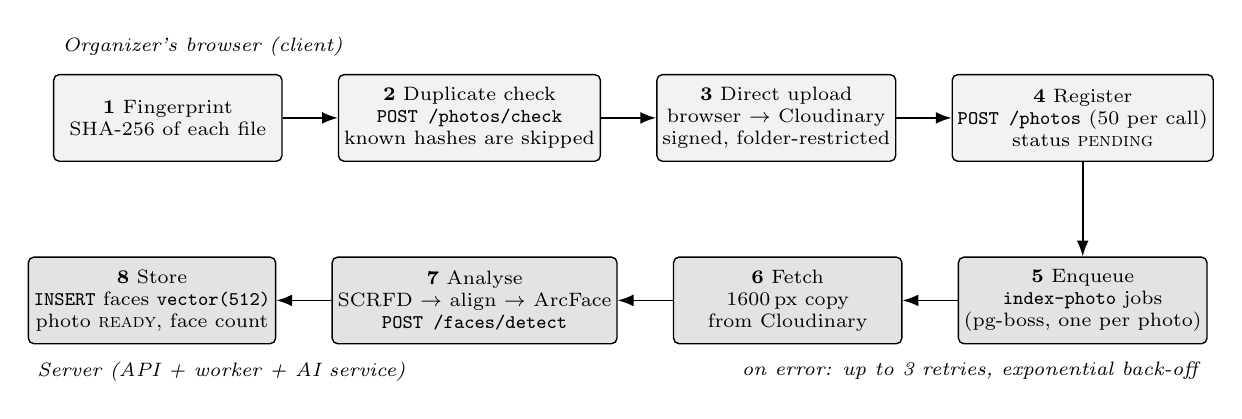
\begin{tikzpicture}[
  font=\scriptsize, >=Latex, node distance=5mm and 7mm,
  stp/.style={draw, rounded corners=2pt, align=center, minimum height=11mm, minimum width=29mm, inner sep=2pt, fill=white, line width=0.5pt},
  cl/.style={stp, fill=gray!10},
  sv/.style={stp, fill=gray!22},
  note/.style={font=\scriptsize\itshape, align=center},
  flow/.style={->, line width=0.6pt}]

% row 1: organizer's browser
\node[cl] (a) {\textbf{1} Fingerprint\\SHA-256 of each file};
\node[cl, right=of a] (b) {\textbf{2} Duplicate check\\\texttt{POST /photos/check}\\known hashes are skipped};
\node[cl, right=of b] (c) {\textbf{3} Direct upload\\browser $\rightarrow$ Cloudinary\\signed, folder-restricted};
\node[cl, right=of c] (d) {\textbf{4} Register\\\texttt{POST /photos} (50 per call)\\status \textsc{pending}};

% row 2: server side (right to left so the arrow continues from step 4)
\node[sv, below=12mm of d] (e) {\textbf{5} Enqueue\\\texttt{index-photo} jobs\\(pg-boss, one per photo)};
\node[sv, left=of e] (f) {\textbf{6} Fetch\\1600\,px copy\\from Cloudinary};
\node[sv, left=of f] (g) {\textbf{7} Analyse\\SCRFD $\rightarrow$ align $\rightarrow$ ArcFace\\\texttt{POST /faces/detect}};
\node[sv, left=of g] (h) {\textbf{8} Store\\\texttt{INSERT} faces \texttt{vector(512)}\\photo \textsc{ready}, face count};

\draw[flow] (a) -- (b); \draw[flow] (b) -- (c); \draw[flow] (c) -- (d);
\draw[flow] (d) -- (e); \draw[flow] (e) -- (f); \draw[flow] (f) -- (g); \draw[flow] (g) -- (h);

\node[note, above=1mm of a.north west, anchor=south west] {Organizer's browser (client)};
\node[note, below=1mm of h.south west, anchor=north west] {Server (API + worker + AI service)};
\node[note, below=1mm of e.south east, anchor=north east] {on error: up to 3 retries, exponential back-off};
\end{tikzpicture}
}
\caption{Photo ingestion pipeline. Steps 1--4 run in the organizer's browser, steps 5--8 on the server.}
\label{fig:index}
\end{figure*}

\subsection{Guest search through messengers}
An event is identified by an eight-character code drawn from 31 unambiguous symbols ($31^8\approx 8.5\times10^{11}$ codes). The guest page opens WhatsApp or Telegram with the code prefilled; the guest sends a selfie (Fig.~\ref{fig:search}). Telegram webhooks are authenticated with a secret header and WhatsApp webhooks with an HMAC-SHA-256 signature compared in constant time. A shared conversation module implements the dialogue once, while the two platform adapters only parse incoming messages and send replies. The selfie is processed in memory; only its embedding is stored on the search record, because the liveness gate needs it later (Section~\ref{sec:liveness}). The reply contains a link to the guest's private gallery.

\begin{figure*}[!t]
\centering
\resizebox{0.78\textwidth}{!}{% Guest search sequence (double-column figure).
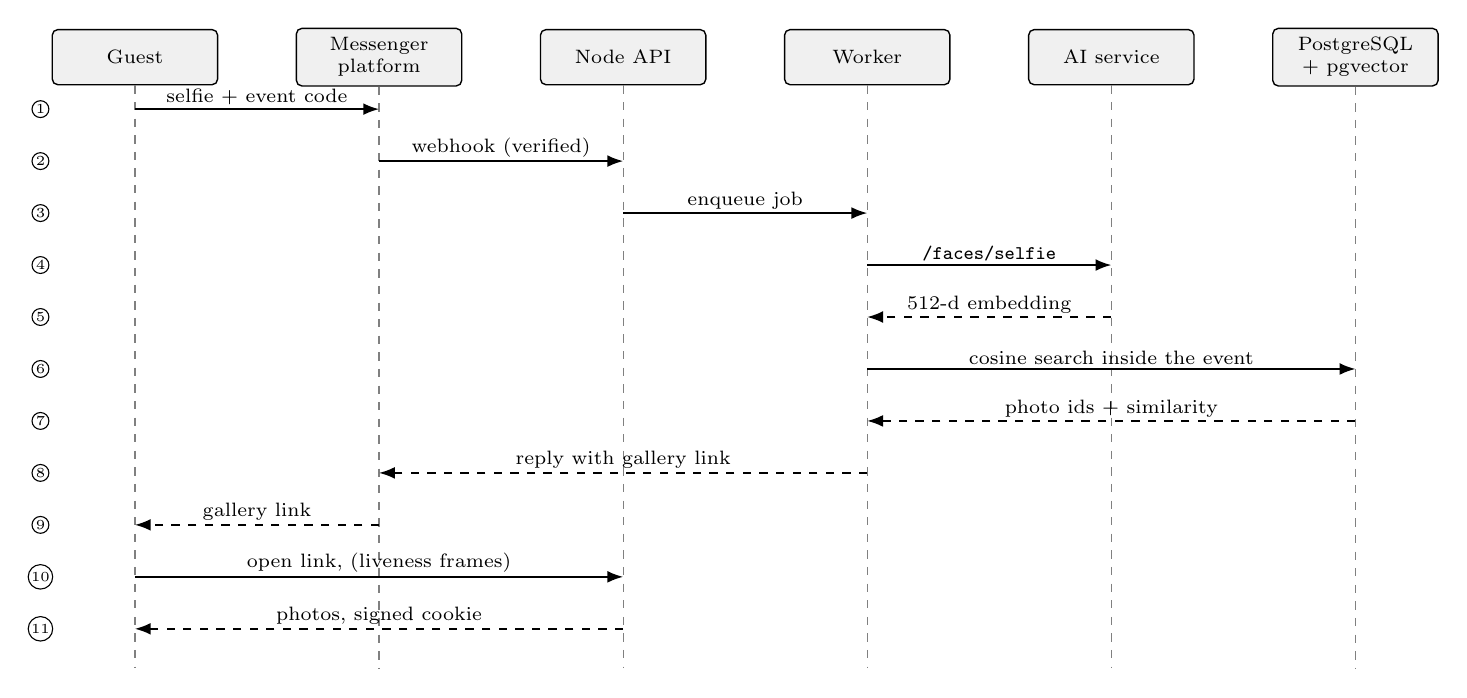
\begin{tikzpicture}[
  font=\scriptsize, >=Latex,
  actor/.style={draw, rounded corners=2pt, minimum width=21mm, minimum height=7mm, align=center, fill=gray!12, line width=0.5pt},
  life/.style={dashed, gray, line width=0.4pt},
  msg/.style={->, line width=0.6pt},
  ret/.style={->, dashed, line width=0.6pt}]

\newcommand{\msg}[5]{\draw[#5] (#2,-#1*6.6mm) -- node[above, inner sep=1.2pt, pos=0.5] {#4} (#3,-#1*6.6mm);
  \node[circle, draw, inner sep=0.5pt, fill=white, font=\tiny] at (-1.2,-#1*6.6mm) {#1};}

\node[actor] (g)   at (0,0)    {Guest};
\node[actor] (p)   at (3.1,0)  {Messenger\\platform};
\node[actor] (api) at (6.2,0)  {Node API};
\node[actor] (w)   at (9.3,0)  {Worker};
\node[actor] (ai)  at (12.4,0) {AI service};
\node[actor] (db)  at (15.5,0) {PostgreSQL\\+ pgvector};
\foreach \n in {g,p,api,w,ai,db} { \draw[life] (\n.south) -- ++(0,-7.4); }

\msg{1}{0}{3.1}{selfie + event code}{msg}
\msg{2}{3.1}{6.2}{webhook (verified)}{msg}
\msg{3}{6.2}{9.3}{enqueue job}{msg}
\msg{4}{9.3}{12.4}{\texttt{/faces/selfie}}{msg}
\msg{5}{12.4}{9.3}{512-d embedding}{ret}
\msg{6}{9.3}{15.5}{cosine search inside the event}{msg}
\msg{7}{15.5}{9.3}{photo ids + similarity}{ret}
\msg{8}{9.3}{3.1}{reply with gallery link}{ret}
\msg{9}{3.1}{0}{gallery link}{ret}
\msg{10}{0}{6.2}{open link, (liveness frames)}{msg}
\msg{11}{6.2}{0}{photos, signed cookie}{ret}
\end{tikzpicture}
}
\caption{Guest search sequence. Steps 10--11 show the visit to the gallery link, with liveness frames when the event requires them.}
\label{fig:search}
\end{figure*}

\subsection{Organizer features}
Organizers sign in with e-mail (verified) or Google. They can invite co-organizers, enable a contributor upload link whose photos stay hidden until approved, switch guest search and liveness on or off, and delete the event. The query in \eqref{eq:match} therefore filters on the approval flag.

% =====================================================================================
\section{Face Analysis and Matching}\label{sec:face}
\subsection{Detection}
SCRFD (\texttt{det\_10g}) \cite{guo2022scrfd} receives the photo scaled to fit a $640\times640$ canvas with its aspect ratio preserved. It predicts, at strides 8, 16 and 32 with two anchors per grid point, a face score, box distances and five landmarks. Detections with score $\ge0.5$ are decoded and merged by non-maximum suppression (IoU $0.4$).

\subsection{Alignment and embedding}
The five landmarks are mapped to the ArcFace template by a least-squares similarity transform \cite{umeyama1991}, the face is warped to $112\times112$ pixels, and an ArcFace ResNet-50 trained on WebFace600K produces a 512-dimensional vector that is L2-normalized \cite{deng2022arcface,insightface}. Because vectors have unit length, cosine similarity is a dot product, and PostgreSQL's cosine distance operator \texttt{<=>} returns $1-q^{\top}\phi(f)$.

\subsection{An ONNX Runtime port}\label{sec:onnx}
The reference \texttt{insightface} Python package compiles C++ extensions during installation, which fails on many Windows machines (goal G6). We therefore re-implemented the pre- and post-processing around the published ONNX files with only ONNX Runtime, OpenCV and NumPy. On 11 test images the port found the same faces and boxes as the reference package and produced embeddings with cosine similarity $\ge0.999999$ to it; yaw estimates agreed within about $2^\circ$.

\subsection{Selfie handling}
A selfie must contain one clear main face. If a second face has at least $60\%$ of the main face's area, the system refuses to guess whom the guest means and asks for another picture. Smaller background faces are ignored.

\subsection{Exact event-scoped search}
For a query $q$, the database evaluates \eqref{eq:match} (Fig.~\ref{fig:sql}) for the rows of one event: the \texttt{event\_id} index selects its faces, the distance operator scores them, a threshold keeps the matches, and \texttt{GROUP BY photo} keeps the best face per photo. The cost is $O(n_E\,d)$ for $n_E$ faces in the event and $d=512$, and, as measured in Section~\ref{sec:eval}, nearly independent of the number of other events. We chose this exact strategy over an approximate index because events contain at most a few tens of thousands of faces and because approximate indexes can silently miss matches (Section~\ref{sec:eval}); a guest who is told ``no photos found'' when photos exist is a failure the design should avoid.

\begin{figure}[!t]
\centering
\scriptsize
\begin{minipage}{0.99\columnwidth}
\begin{verbatim}
SELECT f.photo_id,
       MAX(1 - (f.embedding <=> :q))  AS similarity
FROM   face f JOIN photo p ON p.id = f.photo_id
WHERE  f.event_id = :event AND p.approved
  AND  1 - (f.embedding <=> :q) >= :tau   -- 0.45
GROUP  BY f.photo_id
ORDER  BY similarity DESC  LIMIT 1000;
\end{verbatim}
\end{minipage}
\caption{The matching query of \eqref{eq:match}: exact cosine search restricted to one event (simplified from the production code).}
\label{fig:sql}
\end{figure}


% =====================================================================================
\section{Liveness-Gated Private Delivery}\label{sec:liveness}
\subsection{Threat model}
For a private event, the organizer wants to prevent three things: (a) a recipient who forwards or leaks a gallery link, (b) a person who holds up another person's printed photograph or a screen to the camera, and (c) a person who submits somebody else's photograph as the original selfie in order to obtain that person's photos. Presentation attacks that inject synthetic video into the camera pipeline, high-quality 3-D masks and collusion with the genuine guest are out of scope.

\subsection{Protocol}
Figure~\ref{fig:liveness} summarizes the protocol. The browser guides the guest through tips, a face-in-oval alignment step and a ready button, followed by a three-second countdown. It then captures a burst of 4 frames while the guest looks straight at the camera and a burst of 12 frames, 300\,ms apart, while the guest turns their head. A first prototype that captured one frame at the end of a countdown rejected real users who turned slowly. Burst capture removes the timing requirement: the server keeps the most frontal frame and the most turned frame of the two bursts and ignores the rest.

\begin{figure*}[!t]
\centering
\resizebox{0.97\textwidth}{!}{% Liveness protocol (double-column figure).
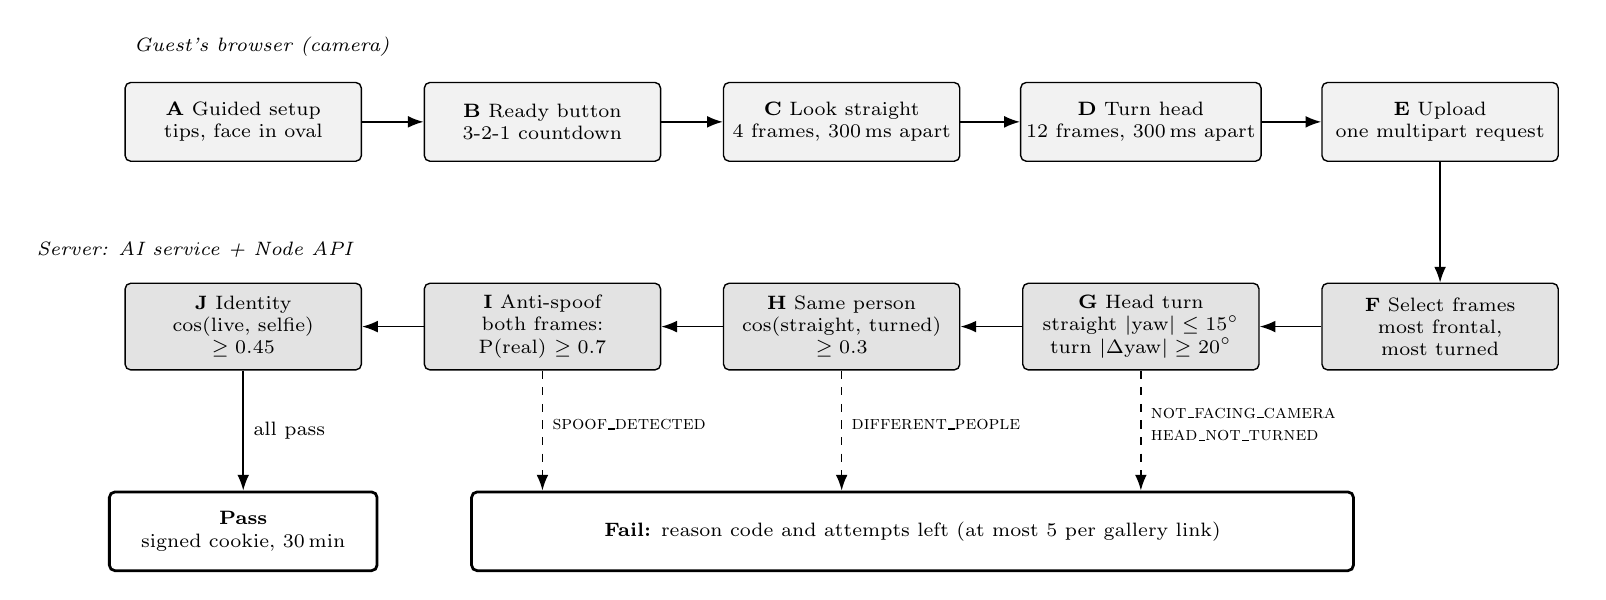
\begin{tikzpicture}[
  font=\scriptsize, >=Latex,
  st/.style={draw, rounded corners=2pt, align=center, minimum height=10mm, minimum width=30mm, inner sep=2pt, fill=gray!10, line width=0.5pt},
  ck/.style={draw, rounded corners=2pt, align=center, minimum height=11mm, minimum width=30mm, inner sep=2pt, fill=gray!22, line width=0.5pt},
  ok/.style={draw, rounded corners=2pt, align=center, minimum height=10mm, inner sep=3pt, fill=white, line width=1pt},
  flow/.style={->, line width=0.6pt},
  note/.style={font=\scriptsize\itshape, align=left}]

% client row (left to right)
\node[st] (c1) at (0,0)    {\textbf{A} Guided setup\\tips, face in oval};
\node[st] (c2) at (3.8,0)  {\textbf{B} Ready button\\3-2-1 countdown};
\node[st] (c3) at (7.6,0)  {\textbf{C} Look straight\\4 frames, 300\,ms apart};
\node[st] (c4) at (11.4,0) {\textbf{D} Turn head\\12 frames, 300\,ms apart};
\node[st] (c5) at (15.2,0) {\textbf{E} Upload\\one multipart request};

% server row (right to left)
\node[ck] (s1) at (15.2,-2.6) {\textbf{F} Select frames\\most frontal,\\most turned};
\node[ck] (s2) at (11.4,-2.6) {\textbf{G} Head turn\\straight $|\mathrm{yaw}|\le 15^\circ$\\turn $|\Delta\mathrm{yaw}|\ge 20^\circ$};
\node[ck] (s3) at (7.6,-2.6)  {\textbf{H} Same person\\cos(straight, turned)\\$\ge 0.3$};
\node[ck] (s4) at (3.8,-2.6)  {\textbf{I} Anti-spoof\\both frames:\\P(real) $\ge 0.7$};
\node[ck] (s5) at (0,-2.6)    {\textbf{J} Identity\\cos(live, selfie)\\$\ge 0.45$};

% outcomes
\node[ok, minimum width=34mm] (pass) at (0,-5.2) {\textbf{Pass}\\signed cookie, 30\,min};
\node[ok, minimum width=112mm] (fail) at (8.5,-5.2) {\textbf{Fail:} reason code and attempts left (at most 5 per gallery link)};

\draw[flow] (c1) -- (c2); \draw[flow] (c2) -- (c3); \draw[flow] (c3) -- (c4); \draw[flow] (c4) -- (c5);
\draw[flow] (c5) -- (s1);
\draw[flow] (s1) -- (s2); \draw[flow] (s2) -- (s3); \draw[flow] (s3) -- (s4); \draw[flow] (s4) -- (s5);
\draw[flow] (s5) -- node[right, pos=0.5] {all pass} (pass);

\draw[flow, dashed] (s2.south) -- node[right, pos=0.45, align=left] {\textsc{not\_facing\_camera}\\\textsc{head\_not\_turned}} (s2.south |- fail.north);
\draw[flow, dashed] (s3.south) -- node[right, pos=0.45] {\textsc{different\_people}} (s3.south |- fail.north);
\draw[flow, dashed] (s4.south) -- node[right, pos=0.45] {\textsc{spoof\_detected}} (s4.south |- fail.north);

\node[note, anchor=south west] at ([yshift=2mm]c1.north west) {Guest's browser (camera)};
\node[note, anchor=south west] at ([yshift=8.5mm]s1.north east) {};
\node[note, anchor=north west] at ([yshift=-2mm]s5.south east) {};
\node[note, anchor=south east] at ([yshift=2mm]s5.north east) {Server: AI service + Node API};
\end{tikzpicture}
}
\caption{Liveness protocol. The client captures two bursts; the server selects two frames and applies five checks in order. Any failing check returns a machine-readable reason and consumes one of five attempts.}
\label{fig:liveness}
\end{figure*}

\subsection{Checks}
\textbf{Head turn.} A 3-D 68-landmark network yields the line between the outer eye corners; seen from the front it lies in the image plane, and a turned head gives it depth. The yaw is the angle between the line and the image plane,
\begin{equation}
\theta=\operatorname{atan2}\!\big(\Delta z,\ \sqrt{\Delta x^{2}+\Delta y^{2}}\big),
\label{eq:yaw}
\end{equation}
which is insensitive to head tilt. The straight frame must satisfy $|\theta_f|\le15^\circ$ and the turned frame must differ by at least $20^\circ$. A printed photograph cannot satisfy the second condition.
\textbf{Same person.} The embeddings of the two frames must have cosine similarity $\ge0.3$; this bar is lower than the match threshold because a turned face looks less similar. It prevents showing one person's face in one burst and another's in the second.
\textbf{Anti-spoofing.} Two MiniFASNet networks (V2 with a $2.7\times$ crop and V1SE with a $4.0\times$ crop around the face, both $80\times80$ input) output a probability that the face is real \cite{minivision}. The two outputs are averaged per frame, and the smaller value of the two frames must be $\ge0.7$.
\textbf{Identity.} Finally, the API compares the live embedding with the selfie embedding stored on the search; the cosine similarity must reach $\tau=0.45$. This step closes threat (c): an attacker who supplies a victim's photograph as the selfie cannot later pass the camera check with their own face.

\subsection{Session handling}
After a pass the API sets a signed, \texttt{httpOnly} cookie that is valid for 30 minutes on that browser only. Each gallery link allows five attempts; further attempts are refused until the guest sends a new selfie. Liveness requests are rate limited. All thresholds are configuration values.

% =====================================================================================
\section{Experimental Evaluation}\label{sec:eval}
\subsection{Scope and setup}
We evaluate the shipped code, not a research prototype. Measurements ran on a virtual machine with four cores of an Intel Xeon processor at 2.30\,GHz and 15\,GiB of memory (Linux 6.18, no GPU), with Python 3.12, ONNX Runtime 1.23.2, OpenCV 4.12, PostgreSQL 16.15 and pgvector 0.6.0. Latencies are medians over repeated runs after warm-up with the 5th and 95th percentiles; all raw results are in the repository (\texttt{paper/data}). \emph{No public identity-labelled benchmark could be downloaded in our build environment, so we did not re-measure recognition accuracy on LFW, IJB-C or a presentation-attack dataset.} Instead, Section~\ref{sec:reported} cites the accuracy reported for the underlying models by their authors, and the remaining subsections measure properties that do not need a large labelled dataset: cost, stability of the embedding under controlled degradations, behaviour at scale, and functional correctness. The limits of this design are discussed in Section~\ref{sec:discussion}.

\subsection{Reported accuracy of the underlying models}\label{sec:reported}
Table~\ref{tab:reported} lists published accuracies. These numbers come from the cited sources, were obtained on different training sets and protocols, and are not our measurements; they indicate the capability of the model family we deploy rather than the performance of our port, which we verified only for equivalence to the reference implementation (Section~\ref{sec:onnx}).

\begin{table}[!t]
\caption{Accuracy on LFW as reported by the original authors, and the reported results of the model pack used in this work. Not measured by us. The buffalo\_l pack also reports CFP-FP 99.33, AgeDB-30 98.23 and IJB-C (E4) 97.25 \cite{insightface}.}
\label{tab:reported}
\centering
\small
\setlength{\tabcolsep}{5pt}
\begin{tabular}{@{}llc@{}}
\toprule
Method & Source & LFW acc. (\%)\\
\midrule
DeepFace & \cite{taigman2014} & 97.35\\
FaceNet & \cite{schroff2015} & 99.63\\
SphereFace (CASIA-WebFace) & \cite{liu2017sphereface} & 99.42\\
CosFace & \cite{wang2018cosface} & 99.73\\
\textbf{buffalo\_l (SCRFD + ArcFace R50)} & \cite{insightface} & \textbf{99.83}\\
\bottomrule
\end{tabular}
\end{table}

\subsection{Cost of the analysis pipeline}
Figure~\ref{fig:latency}(a) breaks down the cost on a six-face photo scaled to 1,600\,px (the size the worker sends). The detector takes 66.9\,ms per photo and ArcFace 64.6\,ms per face, whereas JPEG decoding (5.6\,ms), head pose (14.0\,ms) and the two anti-spoofing networks (6.1\,ms) are small. Whole-photo analysis took 175.8\,ms for a one-face selfie and 508.7\,ms for the six-face photo, consistent with $t\approx0.11\,\mathrm{s}+0.067\,\mathrm{s}\times n_{\mathrm{faces}}$. Extrapolating this model, indexing a 5{,}000-photo event with four faces per photo would take about 31 minutes in one process; we did not run an end-to-end indexing job of that size. Figure~\ref{fig:latency}(b) shows that cost does not depend on the input resolution because the detector input is fixed at $640\times640$ and the recognizer sees $112\times112$ crops: all six faces were found at every size from 320 to 2,560\,px, with the smallest face 24\,px wide at 320\,px.

\begin{figure}[!t]
\centering
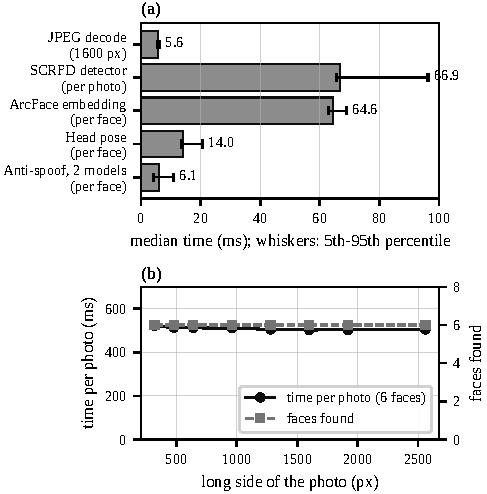
\includegraphics[width=0.86\columnwidth]{figures/graph_latency.pdf}
\caption{(a) Median cost of each pipeline stage at 1,600\,px. (b) Time per photo and faces found for one six-face photo at different resolutions.}
\label{fig:latency}
\end{figure}

\subsection{Stability of the embedding under degradation}
\textbf{Design.} We collected nine identities: the six people of a public group photograph, a sample selfie and two public portraits. Each image was scaled so that the face is 160\,px wide, one degradation at a time was applied to the whole image, the face was detected again, and its embedding was compared with the clean embedding of the same identity. The same perturbed embedding was also compared with the clean embeddings of the eight other identities. This is a stress test of the pipeline's stability, \emph{not} a measure of recognition accuracy across poses, ages or sessions.

\textbf{Reference values.} Clean embeddings of different identities had mean similarity $0.016\pm0.067$ (36 pairs, maximum $0.197$), whereas three different photographs of one person scored $0.73$--$0.78$. The threshold $\tau=0.45$ lies in the gap between the two groups.

\textbf{Results.} Figure~\ref{fig:robust} shows the similarity to the clean face. All nine faces were detected in every condition of the six sweeps and stayed above $\tau$ up to Gaussian blur $\sigma=6$\,px (mean 0.65), JPEG quality 8 (mean 0.83), brightness reduced to 8\% (mean 0.84), noise $\sigma=45$ gray levels (mean 0.75), rotation up to $45^\circ$ (mean 0.92), and 45\% of the lower face covered (mean 0.66). Falling below $\tau$ occurred at the next severity: blur $\sigma=8$ (7 of 9 accepted), noise $\sigma=60$ (8 of 9), rotation $60^\circ$ (8 of 9, minimum 0.40) and 60\% lower-face coverage (3 of 9). Across the 3{,}280 comparisons between a perturbed face and a different identity, the largest similarity was 0.238 and none reached $\tau$.

\begin{figure*}[!t]
\centering
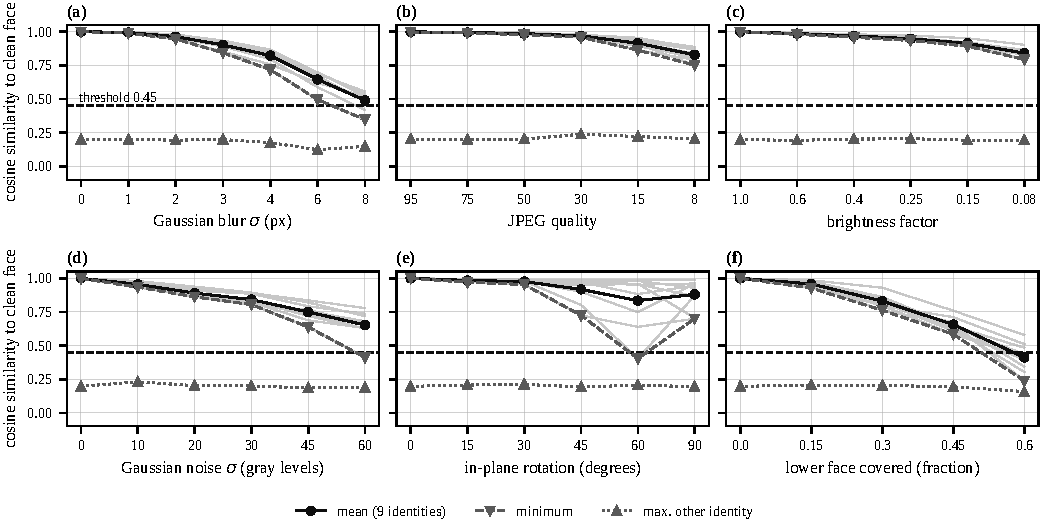
\includegraphics[width=0.97\textwidth]{figures/graph_robustness.pdf}
\caption{Cosine similarity between a degraded face and the clean face of the same identity (thin lines: nine identities; thick: mean) and the largest similarity to any other identity (dotted). The dashed line is the decision threshold 0.45.}
\label{fig:robust}
\end{figure*}

\textbf{Small faces.} Group photographs contain small faces. We placed each identity at decreasing sizes inside a 1,600\,px-wide canvas (Fig.~\ref{fig:size}). Down to 36\,px all nine faces were detected and accepted; at 28\,px 8 of 9 were detected, and at 20\,px only 6 of 9 were detected and 5 accepted. Faces smaller than about 30\,px in a 1,600\,px photo should therefore be considered unreliable. This is consistent with the observation that tiny faces need dedicated treatment \cite{hu2017tinyfaces}.

\begin{figure}[!t]
\centering
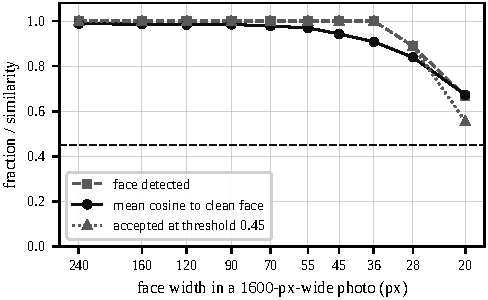
\includegraphics[width=0.86\columnwidth]{figures/graph_face_size.pdf}
\caption{Effect of face size in a 1,600\,px-wide photo on detection, similarity and acceptance (nine identities).}
\label{fig:size}
\end{figure}

\subsection{Vector search}
\textbf{Method.} We generated synthetic embeddings so that cost and recall could be measured at sizes for which no labelled data exists. Each event has identity clusters of eight unit vectors in $\mathbb{R}^{512}$ with mutual cosine similarity between about 0.36 and 0.81; different identities are random directions. A query is a noisy copy of an identity (cosine 0.8 to the identity centre). Each event query returns about eight photos on average. Queries used the production SQL, including the join with the approval flag.

\textbf{Exact event-scoped search.} Figure~\ref{fig:vector}(a) shows median latency growing close to linearly with event size: 1.1\,ms for 500 faces, 2.1\,ms for 1,000, 23.6\,ms for 10,000 and 244\,ms for 100,000 faces. Panel (b) shows that a 10,000-face event took 16.2\,ms in a 50,000-face table and 22.9\,ms in a 500,000-face table, so a tenfold larger table raised the latency by about 41\% while the event size was unchanged: the cost is governed mainly by the size of the event rather than by the total number of stored faces.

\textbf{HNSW versus exact.} Table~\ref{tab:hnsw} compares a global HNSW index ($m=16$, \texttt{ef\_construction}=64) with exact scans of the whole table. HNSW is 5 to 40 times faster than the exact scan but loses matches as the table grows. At 250,000 faces, recall of the matching set was 0.66, 0.83, 0.89 and 0.93 for \texttt{ef\_search} 40, 100, 200 and 400, and some individual queries retrieved none of their true matches. Recall improves with \texttt{ef\_search} and falls with table size (Fig.~\ref{fig:vector}(c)). Random high-dimensional clusters are a hard case for graph indexes, so real embeddings may do better, but the experiment shows why we do not depend on an approximate index for a feature whose failure mode is ``your photos are missing''.

\begin{figure*}[!t]
\centering
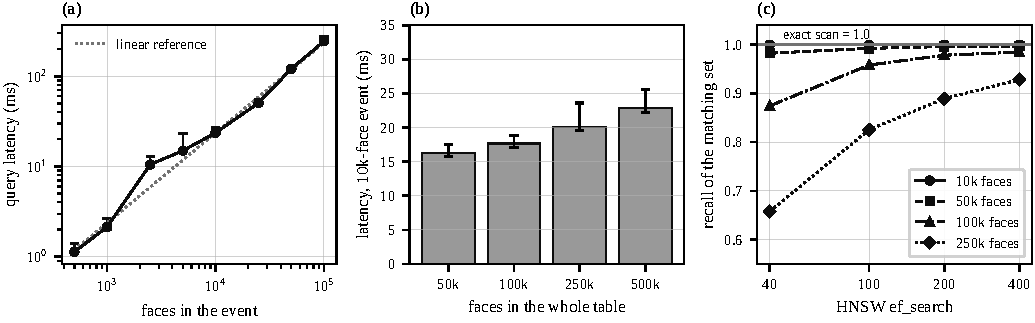
\includegraphics[width=0.97\textwidth]{figures/graph_vector_search.pdf}
\caption{(a) Exact event-scoped query latency versus event size (log--log; whiskers 5th--95th percentile). (b) Latency for a 10,000-face event versus total table size. (c) Recall of the matching set for a global HNSW index versus \texttt{ef\_search} and table size.}
\label{fig:vector}
\end{figure*}

\begin{table}[!t]
\caption{Global top-100 search over synthetic embeddings: exact scan versus HNSW (median latency; recall of faces with similarity $\ge0.45$; 100 queries per table for HNSW, 30 for the exact scan).}
\label{tab:hnsw}
\centering
\small
\setlength{\tabcolsep}{4pt}
\begin{tabular}{rrrrrrr}
\toprule
& Exact & \multicolumn{2}{c}{HNSW, ef=100} & \multicolumn{2}{c}{HNSW, ef=400} & Index\\
Faces & ms & ms & recall & ms & recall & MB\\
\midrule
10{,}000  & 14.7 & 2.0 & 1.000 & 4.9 & 1.000 & 26\\
50{,}000  & 102.0 & 4.1 & 0.993 & 11.7 & 0.998 & 130\\
100{,}000 & 230.6 & 7.1 & 0.958 & 20.3 & 0.985 & 260\\
250{,}000 & 395.8 & 10.1 & 0.826 & 28.6 & 0.928 & 651\\
\bottomrule
\end{tabular}
\end{table}

\textbf{HNSW with an event filter.} PhotoMatch restricts every query to one event. We tested a filtered HNSW query on the 250,000-face table, which holds 250 events. With the \texttt{event\_id} index present, the planner chose an exact plan on its own (recall 1.00, 2.2--2.7\,ms for a 1,000-face event). When we removed that index inside a rolled-back transaction to force the HNSW plan, the filter was applied after the index scan: for 100 requested rows the query returned on average 5.5, 7.3 and 9.4 rows and recalled 0.66, 0.85 and 0.94 of the true matches for \texttt{ef\_search} 40, 100 and 400. This post-filtering behaviour is the reason newer pgvector releases add iterative scans \cite{pgvector08}; we used release 0.6.0, so the experiment documents the failure mode rather than the current behaviour of the extension.

\subsection{Liveness stage}
\textbf{Sanity check on two samples.} We scored the two public samples released with the MiniFASNet project, a live selfie and a phone photograph of a printed poster \cite{minivision}. The live selfie obtained P(real) of 0.9999 (V2) and 0.99999 (V1SE), average 0.99996; the print obtained 0.0044 and 0.305, average 0.155, below the 0.7 threshold. This is a smoke test with $n=2$ and in-distribution samples; it is \emph{not} an estimate of the attack-presentation or bona fide classification error rates defined in ISO/IEC 30107-3 \cite{iso30107}, which require a labelled protocol such as OULU-NPU \cite{boulkenafet2017oulu} or CelebA-Spoof \cite{zhang2020celebaspoof}.

\textbf{Genuine users in poor conditions.} Applying the same degradations to the live selfie, the average P(real) stayed at or above 0.89 for brightness down to 8\%, blur up to $\sigma=6$\,px, JPEG quality down to 8 and face widths from 320 to 36\,px (minimum 0.893 at $\sigma=6$); no genuine sample would have been rejected. With a single identity this says little about the false-rejection rate across devices and skin tones.

\textbf{Cost.} The anti-spoofing networks cost 4.6\,ms per face. Selecting the frames of one complete attempt (16 copies of a $640\times480$ frame, standing in for 4 + 12 webcam frames; detection with head pose on every frame and embedding of the two selected frames) took 2.16\,s (5th--95th percentile 2.04--2.27\,s) in the AI service, and the two anti-spoofing evaluations add about 9\,ms. This is the wait the guest experiences in addition to network time.

\subsection{Throughput of the AI service}
We sent the six-face photograph at 1,600\,px to \texttt{POST /faces/detect} from concurrent clients (48 requests per configuration). One process delivered 1.99, 1.96 and 2.00 photos/s with 1, 2 and 4 clients: throughput is flat because the service serializes inference with a lock and each ONNX Runtime session already uses all four cores, so extra clients only add queueing delay (median latency 0.50, 1.02 and 2.00\,s). Starting more server processes \emph{lowered} throughput (1.32 photos/s with two processes and two clients, 1.14--1.20 with four), which we attribute to thread oversubscription on four cores; we did not test per-process thread limits. On this hardware the practical way to scale indexing is therefore more machines, not more processes. A one-face selfie costs about 0.18\,s of AI time, but because guest searches share this service with indexing, a guest who writes while a large album is being indexed waits behind the backlog; a separate service instance or queue priority for selfies would remove that coupling (not implemented).

\begin{figure}[!t]
\centering
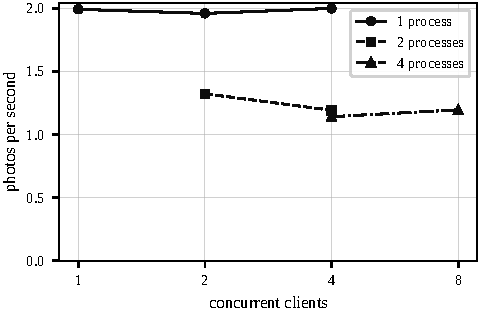
\includegraphics[width=0.86\columnwidth]{figures/graph_throughput.pdf}
\caption{Throughput of the AI service for a six-face 1,600\,px photograph versus concurrent clients and server processes (four CPU cores).}
\label{fig:throughput}
\end{figure}

\subsection{Functional testing}
Three automated suites guard the implementation. A harness with 42 end-to-end checks exercises the real API, worker, database and AI models with the external messengers and object store replaced by local stand-ins: sign-up and e-mail verification, photo indexing, Telegram and WhatsApp flows including signature verification, correct matches, each liveness rejection reason, forged cookies, attempt lockout, duplicate photos and organizer controls. It passed 42 of 42 checks on the final code; it predates the co-organizer and contributor-link features, whose access rules are covered by the API's 18 unit tests (event progress, event codes, message parsing, webhook signatures, access rules and e-mail escaping). The AI service has 15 tests with the real models, including the live selfie versus printed photograph check. All three suites pass.

% =====================================================================================
\section{Discussion and Limitations}\label{sec:discussion}
\textbf{What the evidence supports.} The measurements support three engineering claims: face analysis is cheap enough for a CPU-only server (about 0.11\,s plus 0.067\,s per face); exact event-scoped search is fast enough for realistic events and, unlike a global HNSW index, never misses matches; and the embedding stage is stable under the degradations typical of event photography, with a wide margin between same-person and different-person similarity in our sample.

\textbf{What it does not support.} First, recognition accuracy was not re-measured on a public benchmark; the numbers in Table~\ref{tab:reported} are those of the original authors. Our robustness study uses nine identities and cannot reveal demographic differences, which are known to exist \cite{buolamwini2018,grother2019frvt}, nor errors across ages, expressions or extreme poses. Second, the vector-search experiment uses synthetic embeddings; absolute recall on real face data may differ. Third, the liveness evidence consists of two samples and a quality sweep on one live selfie; we make no claim about APCER, BPCER or resistance to video replay on screens, which passive models are known to find hard \cite{yu2023survey}. The head-turn requirement blocks static photographs but not a replayed video of the genuine guest turning their head, nor injection attacks \cite{tolosana2020}. Fourth, all timings come from one virtual machine.

\textbf{Privacy and law.} Embeddings are biometric templates and can be inverted to approximate face images \cite{mai2019reconstruction}. PhotoMatch stores no selfie image, ties all face data to the event and deletes it with the event, but a public deployment would still need explicit consent, a retention policy, a privacy notice and an assessment under laws such as the GDPR \cite{gdpr}. The recognition models in the \texttt{buffalo\_l} pack are licensed by their authors for non-commercial research use \cite{insightface}, which is acceptable for a research or hobby deployment but would have to be replaced or licensed for commercial use.

\textbf{Design lessons.} (1) For bounded collections, exact search with a relational filter is simpler and more reliable than an approximate index. (2) Putting the queue in the database removed a service without a measurable cost at this scale, but the single-process AI service, not the database, is what limits indexing speed. (3) Capturing bursts and choosing frames on the server turned an unreliable liveness step into one guests can complete at their own pace.

% =====================================================================================
\section{Conclusion and Future Work}\label{sec:conclusion}
PhotoMatch AI lets a guest obtain their photos from an event album with one selfie, optionally protected by a liveness gate that binds the gallery to the person who sent the selfie. The system keeps data, vectors and jobs in a single PostgreSQL database and runs its neural networks on a CPU. Our measurements show that this design is fast, that its embedding stage is stable under common degradations, and that exact event-scoped search avoids the recall losses of approximate indexes; they also show where it stops being reliable, namely faces below roughly 30\,px, extreme blur or occlusion, and horizontally scaled indexing. Future work, in order of importance, is: evaluating the full pipeline on LFW, IJB-C and an event-like labelled collection with demographic breakdowns; a presentation-attack evaluation following ISO/IEC 30107-3 on OULU-NPU and CelebA-Spoof, including replay attacks; re-testing filtered HNSW with iterative scans in current pgvector releases for events beyond 100,000 faces; per-process thread limits for the AI service; face clustering to build per-person albums automatically \cite{wang2019linkage}; and replacing the non-commercial models with commercially licensed ones.

\section*{Acknowledgment}
The author used an AI assistant (Claude, Anthropic) for software development, running the experiments, literature search and drafting of this manuscript. The source code, experiment scripts and raw measurements are available in the project repository. [Add funding and further acknowledgments as appropriate.]

\bibliographystyle{IEEEtran}
\bibliography{refs}

\end{document}
